% SPDX-FileCopyrightText: 2023 Jean-Sebastian de Wet, Jan-Philipp Kiel, Pascal Mager
% SPDX-License-Identifier: CC-BY-4.0
%
% LLNCS macro package for Springer Computer Science proceedings Version 2.21 of 2022/01/12
%
\documentclass[runningheads]{llncs}
%
\usepackage[T1]{fontenc}
% T1 fonts will be used to generate the final print and online PDFs,
% so please use T1 fonts in your manuscript whenever possible.
% Other font encondings may result in incorrect characters.
%
\usepackage{graphicx}
\renewcommand{\figurename}{Figure}
% Used for displaying a sample figure. If possible, figure files should
% be included in EPS format.
%
% If you use the hyperref package, please uncomment the following two lines
% to display URLs in blue roman font according to Springer's eBook style:
%\usepackage{color}
%\renewcommand\UrlFont{\color{blue}\rmfamily}
%\urlstyle{rm}
%
\usepackage{listings}
\AtBeginDocument{\counterwithin{lstlisting}{section}%
  \renewcommand\thelstlisting{\arabic{lstlisting}}}
\renewcommand{\lstlistingname}{Code Example}
\lstset{
  aboveskip=1em,
  breaklines=true,
  captionpos=b,
  escapeinside=||,
  frame=single,
  numbers=left,
  numbersep=1em,
  numberstyle=\tiny,
  showlines=true,
}
\let\origthelstnumber\thelstnumber
\makeatletter
\newcommand*\Suppressnumber{%
  \lst@AddToHook{OnNewLine}{%
    \let\thelstnumber\relax%
     \advance\c@lstnumber-\@ne\relax%
    }%
}
\newcommand*\Reactivatenumber[1]{%
  \setcounter{lstnumber}{\numexpr#1-1\relax}
  \lst@AddToHook{OnNewLine}{%
   \let\thelstnumber\origthelstnumber%
   \refstepcounter{lstnumber}%
  }%
}
\makeatother
% Used to display Python code.
%
\begin{document}
%
\title{Property-Based Testing of Data Analysis Scripts}
\subtitle{A Focus on Hypothesis for Python}
%\subtitle{Enhancing Reliability in DLR Research}  % Alternative subtitle
%
%\titlerunning{Abbreviated paper title}
% If the paper title is too long for the running head, you can set
% an abbreviated paper title here
%
\author{Jean-Sebastian de Wet \and
  Jan-Philipp Kiel \and
  Pascal Mager}
%
\authorrunning{Group Criterion}
% First names are abbreviated in the running head.
% If there are more than two authors, 'et al.' is used.
%
\institute{University of Cologne, Cologne, Germany\\Group Criterion}
%
\maketitle              % typeset the header of the contribution
%
\begin{abstract}
  This report explores property-based testing (PBT) as a meth\-od to enhance the reliability of data analysis scripts, particularly for research at the German Aerospace Center (DLR) using Python. It outlines challenges with traditional testing in scenarios with diverse data values, emphasising the need for innovative testing approaches. The literature study thoroughly covers PBT, including its history, key concepts, advantages and disadvantages, as well as its classification within the test pyramid. It then focuses on a prototype using Hypothesis for Python, detailing its functionalities, integration with pytest, and unique features. Real-world application is demonstrated through code examples showcasing how Hypothesis strengthens the reliability of data analysis scripts. The report concludes that while PBT shows promise in enhancing software testing, further studies are needed to assess its full potential in research-intensive settings like DLR.

  \keywords{Property-Based Testing \and Data Analysis Scripts \and Hypothesis \and Python \and pytest \and Reliability \and Test Pyramid \and Code Examples \and DLR Research.}
\end{abstract}
%
%
%
\section{Introduction}
In the evolving landscape of data analysis, the complexity and volume of data has grown exponentially~\cite{Taylor2023}, creating unique challenges across various fields. This increase in data complexity requires robust testing methodologies to ensure the accuracy and reliability of data analysis tools and scripts. Traditional testing approaches, which are primarily based on specific input-output cases, often fall short in addressing the dynamic and unpredictable nature of modern datasets. These limitations are particularly evident in specialised fields such as aerospace research, where the volume and variety of data is exceptionally large.

The structure of this report begins with a brief description of the applied methodology, followed by the presentation of results. These results are then discussed in detail, placed in the context of the existing literature and used to derive implications for future works.

\section{Background}
Within the German Aerospace Center (DLR), the reliability of data analysis scripts is a cornerstone of successful research outcomes. DLR researchers frequently use Python~\cite{Kurnatowski2020}, along with powerful libraries like pandas\footnote{pandas is a Python library offering data manipulation and analysis tools} and Matplotlib\footnote{Matplotlib is a Python library for creating visualisations}, for complex data manipulations and visualisations. This introduces significant testing challenges. DLR, being at the forefront of aerospace research and development, deals with an enormous range of data variables, from satellite imagery to flight dynamics.\footnote{https://www.dlr.de/en/dlr/about-us, accessed: 2024-01-21} This variety and complexity of data make testing particularly challenging. This report explores the adoption of property-based testing (PBT), presenting it as an innovative and essential strategy to overcome these testing challenges.

\section{Method}
Our methodology involved two key stages.

\subsection{Literature Study}
The first stage of our methodology involved a thorough literature review on PBT. Our objective was to gain an in-depth understanding of its theoretical foundations, including its history, key principles, and diverse applications. The process consisted of systematic searches in academic databases and online repositories, using targeted keywords such as `property-based testing' and `automatic test case generation'. We focused on selecting literature from various domains, particularly papers highlighting PBT's ability to create diverse test inputs. This approach provided a solid knowledge base and included insights on handling complex datasets at the DLR.

\subsection{Prototyping}
The second stage centered on practical application through the use of Jupyter Notebooks\footnote{Jupyter Notebooks is a web-based interactive computing platform for data analysis}. We developed a comprehensive guide (\texttt{tutorial.ipynb}) for using Hypothesis\footnote{https://hypothesis.works/, accessed: 2024-01-21}---a PBT framework for Python. This guide covered critical aspects including installation, configuration, and integration with pytest\footnote{pytest is a Python testing framework}. It also provided concrete examples demonstrating the process of defining properties and generating test inputs using Hypothesis. To validate our methodology, we conducted a case study (\texttt{data\_analysis.ipynb}) that involved applying PBT to a data analysis script on astronauts. This case study served as a realistic application, illustrating the potential of PBT in complex data scenarios.

\section{Results}
First, we uncovered key theoretical insights about PBT through our literature study presented in this report. Second, we demonstrated the practical effectiveness of Hypothesis in our prototype by using code examples from the Jupyter Notebooks included in the \texttt{code} folder of this repository.

\subsection{Literature Study of Property-Based Testing}
\subsubsection{History}
The origins of PBT can be traced back more than 20 years ago, even before the year 2000. While it had already been a subject within information technology research, as seen in Guo et.~al.~\cite{Guo1999} as well as Fink and Bishop~\cite{Fink1997}, it gained significantly more attention with the development of QuickCheck\footnote{QuickCheck is a PBT tool for the Haskell programming language}~\cite{Shi2023,Guo1999,Fink1997,MacIver2019,Honarvar2020}. Initially focusing on research questions related to topics such as automation of test input generation and automated techniques in general~\cite{Fink1997} and directing the automated input generator towards values with a higher probability of failure~\cite{Loescher2017}, recent papers have focused on the implementation of different frameworks or platforms and techniques for PBT application~\cite{Padhye2019,Honarvar2020,Shi2023,Corgozinho2023}. Moreover, PBT currently enjoys wide-ranging support in different programming languages including automation capabilities~\cite{Chen2022,Padhye2019,Honarvar2020,ElazarMittelman2023,Shi2023}, as well as the application within many different Python projects using Hypothesis~\cite{Corgozinho2023}.

\subsubsection{Key Concepts}
PBT is a method supporting the formal verification of a software~\cite{Chen2022,Fink1997,Honarvar2020,Paraskevopoulou2015}, focusing on validating high-level or general properties of the software~\cite{Fink1997,Honarvar2020,Corgozinho2023}. Test cases within this method are typically formulated using logical descriptions of the expected behavior of the software~\cite{Chen2022,Fink1997,Honarvar2020,Loescher2017,Corgozinho2023}, including pre- and post-conditions of the system~\cite{Honarvar2020}. To formally approximate the system's behavior, a single test case is executed multiple times with randomly generated input to search for counterexamples that violate specific properties or cause a software crash, thereby invalidating said property~\cite{Chen2022,Loescher2017,Padhye2019,ElazarMittelman2023,Paraskevopoulou2015,Corgozinho2023}. Data generators are used for random input generation, which can be adjusted based on a certain domain's needs~\cite{Chen2022,Loescher2017,Padhye2019,ElazarMittelman2023}. Through automated execution of tests with random input, PBT tries to approximate the validity of a property by subjecting it to numerous instantiations within a given input range; otherwise, the property is falsified~\cite{Fink1997,ElazarMittelman2023,Corgozinho2023,Paraskevopoulou2015}. To further elaborate on the properties, which represent the desired behaviour in terms of input and output of given tested functions through specifications~\cite{Chen2022,Fink1997,Loescher2017}, some examples can be given. To start with a simple one, think of a function that adds two numbers (A, B) and returns the sum of both numbers (A+B). You can define a test which asserts that for any given input for either A and B, the function will return the addition of both numbers. Another simple example would be a sort-function. Assume a sort-function sorts a list, the invariant would be, that sorting an already sorted or the same list twice, will result in a sorted and the same list~\cite{Corgozinho2023}. A common example which is frequently used for showcasing PBT are binary search trees~\cite{Corgozinho2023,Shi2023}, where one property to test might be that after ``insert[ing] a key into a valid BST [binary search tree], it should maintain its validity''~\cite{Shi2023}. In the context of PBT you would then use logic expressions for your tests and use a random input generator to check whether the given property is violated in any case within a certain input range. It is also possible to apply it to software security concerns such as authentication~\cite{Fink1997} or for verifying the ``correctness of hardware [and] external software involved''~\cite{Chen2022}. In summary, PBT allows for the approximation of a system's invariants formal verification~\cite{Fink1997,ElazarMittelman2023,Corgozinho2023}.

\subsubsection{Advantages and Disadvantages}
As previously mentioned, PBT supports the formal validation of software by testing specified properties using randomly generated input for each test. However, describing all expected behavior of a system in a logical style is often less feasible~\cite{Chen2022,Koopman2012}. In contrast, by applying PBT the required endeavour for formal validation can be lowered~\cite{Hritcu2016,Chen2022,Paraskevopoulou2015}. Moreover, specifications used for PBT might also improve cooperation between software developers and testers in larger projects, as the language used for defining tests is easier to grasp compared to abstract proofs~\cite{Chen2022,Loescher2017}. Besides this, PBT can also be applied to tests in several contexts~\cite{Karlsson2019}, such as interfaces~\cite{Karlsson2019,Francisco2013,LamelaSeijas2013}, e.g. by testing invariants regarding the responses of requested URLs of REST-APIs~\cite{Karlsson2019}. Other potential domains of application include telecom systems~\cite{Arts2006}, file synchronisation services~\cite{Hughes2016} and databases~\cite{Arts2015}. Despite its wide applicability and advantages regarding formal validation, PBT reduces engineering effort in terms of defining individual test cases and input parameters~\cite{Chen2022,Loescher2017,Corgozinho2023} and may also incentivise developers to design code that can be easily expressed by properties~\cite{Chen2022}. More specifically, when compared to manually written tests like in unit-testing, PBT allows the software engineer to put more emphasis on ensuring and restoring correctness of the software and less on ``defining test case inputs, examples, and scenarios''~\cite{Corgozinho2023}, turning it into a much less mundane effort~\cite{Loescher2017}. It therefore reduces costs related to testing, including costs induced by changes made to the software~\cite{Chen2022,Loescher2017}. Furthermore it allows for validating a software based on a much larger range of inputs~\cite{Loescher2017,Corgozinho2023} and even more creative or sophisticated inputs~\cite{Arts2015}. As such PBT complements traditional testing techniques by unveiling yet unknown bugs within even well tested systems~\cite{Arts2015,Hughes2016,Arts2006} and in general, is useful for finding bugs within the implementation of a software and its specifications~\cite{Chen2022,Fink1997,Loescher2017,Paraskevopoulou2015,Claessen2000,Corgozinho2023}.

Although PBT offers quite some advantages, it does not come without any disadvantages. Due to the randomness of the input generator provided by tools, the chances of finding more specific bugs is reduced, depending on the portion of erroneous inputs of the entire input range, thus potentially failing to unveil errors~\cite{Loescher2017,Padhye2019,ElazarMittelman2023,Shi2023}. It should be noted that processing a large number of tests can lead to reduced efficiency~\cite{ElazarMittelman2023,Shi2023}, as it involves attempting to approximate a formal proof using numerous randomly selected scenarios~\cite{Fink1997,ElazarMittelman2023,Paraskevopoulou2015}. Löscher and Sagonas~\cite{Loescher2017} gave quite a good fictional example using a ``system of network nodes''~\cite{Loescher2017}. They tried to falsify the property that for any input scenarios (graphs created), the longest of the shortest paths ``between the sink and other nodes [...] should not exceed 21 hops''~\cite{Loescher2017}. Even after 100000~tests they were not able to falsify the property, which could be done manually~\cite{Loescher2017}. A possible solution to this problem is implied by the usage of individually conceptualised data generators~\cite{Loescher2017,ElazarMittelman2023,Shi2023,Paraskevopoulou2015,Claessen2000} or targeted property-based testing~\cite{Loescher2017}. While constraining data generators in order to cancel a test by using pre-conditions as a form of domain knowledge represents an option to reduce computation effort~\cite{Loescher2017,ElazarMittelman2023,Shi2023}, targeted property-based testing achieves this by guiding the input generator~\cite{Loescher2017}. The idea is to increase the chance of generating inputs causing the violation of a property, by applying search techniques~\cite{Loescher2017}. However, the first technique of implementing specified data generators comes with its own challenges regarding the development~\cite{Loescher2017,ElazarMittelman2023,Shi2023}, resulting in a reduced attractiveness of PBT.

\subsubsection{Classification within the Test Pyramid}
To position PBT within the test pyramid as depicted in Figure~\ref{fig:test_pyramid}, our focus was on the levels of unit and integration (service) testing~\cite{Aniche2022,Radziwill2020}. Existing literature indicates that PBT has not yet been applied for testing at the highest level of either system or user interface (UI) tests~\cite{Radziwill2020,Aniche2022}, leaving these levels outside the scope of our analysis.

\begin{figure}
  \centering
  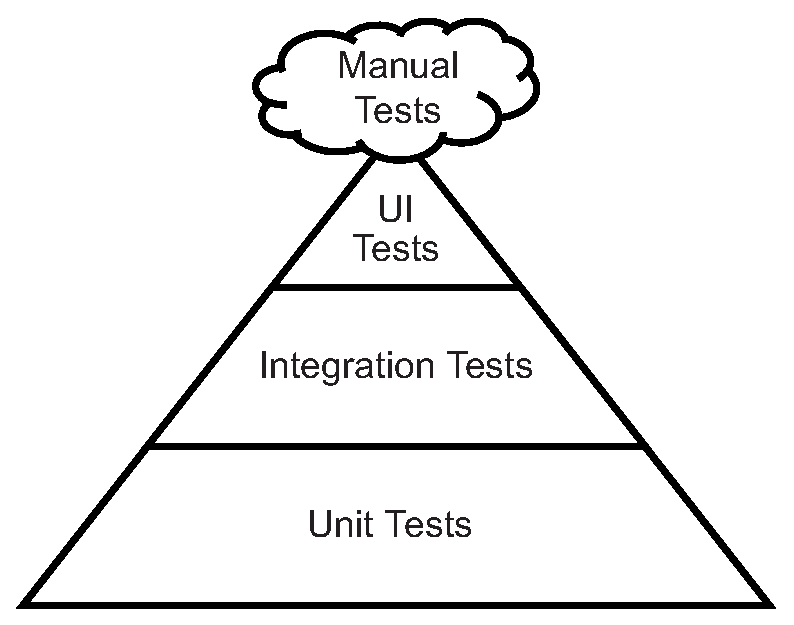
\includegraphics[width=.618\textwidth]{includes/test_pyramid.eps}
  \caption{Test Pyramid. Based on Vocke, H.: The Practical Test Pyramid (2018). https://martinfowler.com/articles/practical-test-pyramid.html}
  \label{fig:test_pyramid}
\end{figure}

Beginning with unit testing, ``developers perform unit testing to ensure that each component correctly implements its design and is ready to be integrated into a system of components''~\cite{Hartmann2000}. In other words, each function or module of a system is tested in an isolated manner. Furthermore it emphasised on ``example-based''~\cite{Corgozinho2023} testing of individual features or functions---also referred to as the ``smallest parts''~\cite{Aniche2022} of a system~\cite{Hartmann2000,Corgozinho2023}.

Within integration tests, as the name suggests, every component of a system is integrated with each other, including relevant external components~\cite{Aniche2022,Hartmann2000,Radziwill2020}. The goal is to ensure that interaction between the given components works correctly and therefore, the combined set of functionality~\cite{Hartmann2000,Aniche2022}.

Although the majority of the use cases explaining how PBT works focus on individual components, such as functions for adding numbers, inserting nodes in binary search trees,
and managing sorted lists, it also offers potential applications concerning the physical and external aspects of software~\cite{Chen2022}. Referring back to the example regarding authentication, one can test not only the authentication functionality of a system but also the integration of its respective authentication services~\cite{Fink1997}. Additionally, PBT has been utilised in various scenarios such as testing RESTful APIs within the context of OpenAPIs\footnote{OpenAPI is a specification for defining and documenting RESTful APIs}~\cite{Karlsson2019}, telecom systems~\cite{Arts2006}, synchronisation services~\cite{Hughes2016} or automotive systems~\cite{Arts2015}. For instance, in the case of QuickREST\footnote{QuickREST is a library for testing and building OpenAPI-described RESTful APIs}, response codes can be used to differentiate between invalid and valid URL requests, ultimately revealing previously unknown `underspecification' in the utilised OpenAPI documentation~\cite{Karlsson2019}. Similarly, in the context of automotive systems, testing correct request processing unveiled a previously unknown bug related to task prioritisation~\cite{Arts2015}. Lastly, complete crashes of addressed components can also be observed~\cite{Arts2006}.

Consequently, the PBT method can be applied to both unit and integration testing. In practical terms, PBT is commonly employed for unit testing and is well suited for this purpose, as its highlighted advantages demonstrate complementary effects compared to simple example-based unit testing. However, its applicability is not restricted solely to unit testing. Existing literature has shown that it also extends to testing the integration of various components.

\subsubsection{Tools and Programming Languages}
As previously mentioned, PBT is widely supported across various programming languages~\cite{Chen2022,Shi2023}. It is supported by Java (QuickTheories\footnote{https://github.com/quicktheories/QuickTheories, accessed: 2024-01-21}), coq (QuickChick\footnote{https://github.com/QuickChick/QuickChick, accessed: 2024-01-21}), Scala (ScalaCheck\footnote{https://scalacheck.org/, accessed: 2024-01-21}), Erlang (PropEr\footnote{https://proper-testing.github.io/, accessed: 2024-01-21}), Haskell (QuickCheck\footnote{https://hackage.haskell.org/package/QuickCheck, accessed: 2024-01-21}), OCaml (QCheck\footnote{https://github.com/c-cube/qcheck/, accessed: 2024-01-21} and Crowbar\footnote{https://github.com/stedolan/crowbar, accessed: 2024-01-21}) to name a few examples~\cite{MacIver2016,Padhye2019,Paraskevopoulou2015,Arts2008,Papadakis2011,Claessen2000}. Obviously many of these were inspired by QuickCheck, being the tool popularising PBT. However, this study focuses on Hypothesis, a Python-based PBT implementation framework. This framework has recently attracted significant attention~\cite{Corgozinho2023,MacIver2019}, is compatible with pytest and unittest\footnote{unittest is Python's built-in testing framework}, as well as being open source under the Mozilla Public License 2.0\footnote{https://hypothesis.works/products/, accessed: 2024-01-21}.

\subsection{Prototype using Hypothesis for Python}
\subsubsection{Overview}
Hypothesis is a Python library for property-based testing, aiming to simplify software testing. Contrary to traditional unit testing, which concentrates on executing a function and asserting specific outcomes, Hypothesis shifts the focus towards ensuring that assertions hold across all data conforming to a predefined specification.

This offers several advantages, inlcuding the identification of edge cases and hidden bugs not typically anticipated in standard testing procedures. The test robustness is enhanced by utilising a wide variety of inputs, some of which are randomly generated. Additionally, it can consolidate multiple traditional unit test cases into a single PBT test case, potentially saving time. Hypothesis also seamlessly integrates with other testing frameworks, such as pytest and nose\footnote{nose is a Python testing framework that extends the built-in unittest library}.

However, there are drawbacks to consider. The execution times for test suites may increase due to Hypothesis generating and executing numerous subordinate test cases. While Hypothesis attempts to reproduce the input leading to test failures, understanding the cause of failure can sometimes be challenging. Moreover, PBT typically offers less control compared to traditional unit tests.\footnote{https://hypothesis.readthedocs.io/en/latest/, accessed: 2024-01-10} These pros and cons align with the general advantages and disadvantages of PBT as discussed in our literature study.

\subsubsection{Strategies and Data Generation}
A central concept within Hypothesis is the utilisation of search strategies. These strategies refer to how Hypothesis will try to generate inputs for test functions. Or rather, wha it will use to search for bugs. For that, Hypothesis is equipped with a diverse set of search strategies, enabling it to generate various types of data, including text, floats, integers, boolean values, values from specified sets, and values conforming to given regular expressions. Furthermore, it is possible to refine these strategies using input parameters. Such refinements can include constraints like limiting the range of generated float values or specifying permissible date ranges.

The implementation of search strategies within Hypothesis adheres to a consistent format. Typically, a search strategy object is instantiated using the syntax \texttt{st.(type)}, where \texttt{type} indicates the desired search strategy, such as \texttt{text}, \texttt{float}, or \texttt{date}. This instantiation process allows for further refinement through the specification of parameters. These parameters can impose constraints, for example, restricting dates to a specified range or generating floats with a maximum size limit. By default, Hypothesis is configured to generate a series of 100 distinct tests for each defined strategy.

\subsubsection{Installation}
In order to use Hypothesis, the package must first be installed using Python's package installer pip. This can be done by executing the command \fbox{\texttt{pip install hypothesis}}. The specific configuration used in this study is described as follows:
\begin{itemize}
  \item Operating System: Ubuntu 22.04.3 LTS
  \item Python Version: 3.10.12
  \item pip Version: 22.0.2
  \item Hypothesis Version: 6.92.2
\end{itemize}
It is worth noting that the Hypothesis team is officially committed to supporting the latest version of Python.\footnote{https://hypothesis.readthedocs.io/en/latest/, accessed: 2024-01-10}

\subsubsection{Usage}
To understand the use of Hypothesis, consider the following basic test shown in Code Example~\ref{lst:basic_test} below. The complete Code Examples \ref{lst:basic_test}--\ref{lst:seeds} can be found in the provided \texttt{tutorial} Jupyter Notebook.
\begin{lstlisting}[language=Python,caption={Basic Test from \texttt{tutorial.ipynb}},label=lst:basic_test]
  from hypothesis import given
  import hypothesis.strategies as st

  @given(st.integers())
  def test_builtin_abs(x: int) -> None:
      assert abs(x) >= 0
      assert abs(x) == (x if x >= 0 else -x)

  test_builtin_abs()
\end{lstlisting}
The primary method of annotating a Hypothesis test involves the \texttt{given} decorator (line~4). This decorator accepts a search strategy object, utilising it to supply values for the function's parameters. In the presented case, integers are generated as inputs for the parameter $x$ in line~5.

The test function then asserts that certain properties hold for each generated value of $x$. In this specific example, the test validates the correct functionality of Python's built-in absolute value function (lines~6--7).

\vspace{5mm}
\noindent Another feature is the ability to create new, specialised search strategies. The following Code Example~\ref{lst:complex_inputs} illustrates the creation of complex inputs:

\begin{lstlisting}[language=Python,caption={Complex Inputs from \texttt{tutorial.ipynb}},label=lst:complex_inputs]
  from hypothesis.strategies import composite

  PI = 3.14159

  @composite
  def custom_input_generator(draw) -> tuple[float, str]:
    decimal = draw(st.floats(max_value=PI))
    text = draw(
      st.text(alphabet=st.characters
          (whitelist_categories=['Lu']),
          min_size=2, max_size=5))
    return decimal, text

  @given(custom_input_generator())
  def test_custom_input_generator
        (generated_input: tuple[float, str]) -> None:
    decimal, text = generated_input
    assert decimal <= PI
    assert len(text) >= 2 and len(text) <= 5
    assert text.isupper()
\end{lstlisting}
The \texttt{composite} decorator (line~5) is utilised to define a function for generating a customised search strategy, achieved by combining existing strategies. In the example above, the float search strategy is used to generate floats with a maximum value of $\pi$ in line~7. Then, the text search strategy is used to create strings consisting solely of uppercase letters (line~10), with a length contraint of 2--5 characters (line~11). The test function (line~14--20) then asserts that the generated decimal and text adhere to the specified structure and constraints.

\vspace{5mm}
\noindent Improving the robustness of tests can be achieved by increasing the number of test cases generated as shown in Code Example~\ref{lst:test_case_amount} below:

\begin{lstlisting}[language=Python,caption={Specifying Test Case Amount from \texttt{tutorial.ipynb}},label=lst:test_case_amount]
  from hypothesis import settings

  @settings(max_examples=100)
  @given(st.integers())
  def test_builtin_abs(x: int) -> None:|\Suppressnumber|
    ...|\Reactivatenumber{9}|

\end{lstlisting}
This approach not only helps to improve test coverage, but also approximates formal verification by generating a large amount of random input. The test quantity generated can be adjusted using the \texttt{settings} decorator in line~3.

To apply this setting globally at the beginning of a Python file, the following approach in Code Example~\ref{lst:settings} can be used:

\begin{lstlisting}[language=Python,caption={Global Settings from \texttt{tutorial.ipynb}},label=lst:settings]
  settings.register_profile("default", max_examples=100)
  settings.load_profile("default")
\end{lstlisting}

\vspace{5mm}
\noindent Another useful feature of Hypothesis is its capability to specify a seed, ensuring reproducibility of test cases as demonstrated in the following Code Example~\ref{lst:seeds}:

\begin{lstlisting}[language=Python,caption={Specifying Seeds from \texttt{tutorial.ipynb}},label=lst:seeds]
  from hypothesis import given, seed
  import hypothesis.strategies as st

  @seed(30)
  @given(st.integers())
  def test_builtin_abs(x: int) -> None:|\Suppressnumber|
  ...|\Reactivatenumber{11}|

\end{lstlisting}
The \texttt{seed} decorator (line~4), along with a designated seed value, is used to set a seed. By setting a seed, Hypothesis generates a consistent set of test cases, thereby eliminating the element of randomness. This is particularly helpful for debugging purposes, as Hypothesis can identify and present the specific seed that led to a failure. Additionally, incorporating specific seeds into a test suite, alongside randomised tests, can enhance testing reliability. 

\subsubsection{Integration with pytest}
The integration of Hypothesis with pytest is seamless. To initiate the testing process, simply run the command \fbox{\texttt{pytest}}, which will automatically detect and run the Hypothesis tests. This automatic detection is exemplified in the included \texttt{tutorial} Jupyter Notebook, where it can be observed that pytest accurately identifies Hypothesis tests. However, it is crucial to recognise that although pytest registers a Hypothesis test as a singular test entity, in reality, it executes multiple underlying tests.

\vspace{5mm}
\noindent For acquiring more in-depth information regarding Hypothesis, the optional flag \texttt{-{}-hypothesis-show-statistics} can be utilised. As shown in the shortened output below, this flag displays detailed information specific to Hypothesis:
\begin{verbatim}
  ==================== Hypothesis Statistics ====================
  test.py::test_builtin_abs:
    - during generate phase (0.02 seconds):
      - Typical runtimes < 1ms, of which < 1ms in data generation
      - 100 passing, 0 failing, 0 invalid examples
    - Stopped because settings.max_examples=100
\end{verbatim}

\subsubsection{Data Analysis Scripts}
Hypothesis is a powerful tool for testing data analysis scripts, especially for validating data preparation and cleaning. Its strength lies in its ability to simulate a wide range of inputs, which increases the robustness of the functions. In the following case study, we examine the application of Hypothesis to an exemplary data analysis script on astronauts provided by Stoffers and Schlauch~\cite{Stoffers2021} from the DLR. The complete Code Examples \ref{lst:calc_age}--\ref{lst:overflow_err} can be found in the included \texttt{data\_analysis} Jupyter Notebook.

\newpage
\noindent The first function covered is \texttt{calculate\_age}, as shown in the Code Example~\ref{lst:calc_age} below. It serves as an auxiliary function in the data preparation script.

\begin{lstlisting}[language=Python,caption={Calculate Age from \texttt{data\_analysis.ipynb}},label=lst:calc_age]
  |\Suppressnumber|
  ...|\Reactivatenumber{7}|
  def calculate_age(born):
    today = date.today()
    return today.year - born.year -
      ((today.month, today.day) < (born.month, born.day))
\end{lstlisting}
It calculates the current age by subtracting the year of birth from the present year (line~9) and adjusts for birthdays not yet occurred in this year (line~10).

The testing of this function is demonstrated in the following Code Example~\ref{lst:test_calc_age}, using the \texttt{test\_calculate\_age} function:

\begin{lstlisting}[language=Python,,caption={Test Calculate Age from \texttt{data\_analysis.ipynb}},label=lst:test_calc_age]
  @given(st.dates(min_value=date(1920, 1, 1), 
                  max_value=date.today()))
  def test_calculate_age(born: date) -> None:
    age = calculate_age(born)
    assert age >= 0
       and age <= (born.today().year - born.year)
  
  test_calculate_age()
\end{lstlisting}
In this test, the \texttt{given} decorator generates random dates between the 1st of January 1920 (line~1) and today (line~2). The function then asserts that the calculated age is non-negative (line~5) and does not exceed the maximum possible age based on the year of birth (line~6). This ensures the correct functionality of the \texttt{calculate\_age} function.

\vspace{5mm}
\noindent The next function \texttt{prepare\_data\_set} is arguably the most important in the script, being responsible for preparing the data sets as shown in Code Example~\ref{lst:prep_data}:

\begin{lstlisting}[language=Python,caption={Prepare Data Set from \texttt{data\_analysis.ipynb}},label=lst:prep_data]
  def prepare_data_set(df):
    df = rename_columns(df)
    df = df.set_index("astronaut_id")

    # Set pandas dtypes for columns with date or time
    df = df.dropna(subset=["time_in_space"])
    df["time_in_space"] = df["time_in_space"].astype(int)
    df["time_in_space"] = pd.to_timedelta(df["time_in_space"], unit="m")
    df["birthdate"] = pd.to_datetime(df["birthdate"])
    df["date_of_death"] = pd.to_datetime(df["date_of_death"])
    df.sort_values("birthdate", inplace=True)

    # Calculate extra columns from the original data
    df["time_in_space_D"] = df["time_in_space"] / pd.Timedelta(days=1)
    df["alive"] = df["date_of_death"].apply(is_alive)
    df["age"] = df["birthdate"].apply(calculate_age)
    df["died_with_age"] = df.apply(died_with_age, axis=1)
    return df|\Suppressnumber|
  ...|\Reactivatenumber{46}|

\end{lstlisting}
Hypothesis is well suited for testing even complex functions. In the above example, the function transforms an astronaut dataset by renaming columns (line~2), managing missing values and data types (lines~6--10), and adding analytical columns (lines~14--17).

The following \texttt{astronaut\_data} function in Code Example~\ref{lst:astro_data} is designed to generate appropriate inputs for the previous \texttt{prepare\_data\_set} function:

\begin{lstlisting}[language=Python,caption={Astronaut Data from \texttt{data\_analysis.ipynb}},label=lst:astro_data]
  @st.composite
  def astronaut_data(draw) -> dict:
    astronaut = draw(st.from_regex(r"http://www\.wikidata\.org/entity/Q\d+", fullmatch=True))
    astronautLabel = draw(st.from_regex(r"[A-Z][a-z]+ [A-Z][a-z]+", fullmatch=True))
    birthdate = draw(st.dates(min_value=date(1920, 1, 1), max_value=date(2030, 12, 31)))
    birthplaceLabel = draw(st.from_regex(r"[A-Z][a-z]+", fullmatch=True))
    sex_or_genderLabel = draw(st.sampled_from(["male", "female"]))
    time_in_space = draw(st.integers(min_value=1, max_value=900)) 
    date_of_death = draw(st.one_of(
        st.none(), 
        st.dates(birthdate + timedelta(days=1), 
                  max_value=date(2030, 12, 31))
        )
    )|\Suppressnumber|
    ...|\Reactivatenumber{40}|

\end{lstlisting}
The \texttt{astronaut\_data} function creates an dictionary with various inputs (lines~1--2). Specifically, it generates an astronaut link and label using \texttt{st.from\_regex} search strategies (lines~3--4), and a birthdate within a specified range using the \texttt{st.dates} strategy (line~5). The sex or gender label is generated using \texttt{st.sampled\_from}, drawing from male and female values (line~7). The time in space is generated using \texttt{st.integers} within a given range (line~8). Additionally, the date of death is generated using \texttt{st.one\_of} to choose between two strategies: \texttt{st.none} for the possibility of no death date (line~10), and \texttt{st.dates} to ensure a date after the birthdate (line~11) and within a realistic timeframe (line~12). This combination of strategies in Hypothesis enables the generation of complex and realistic test data. Through the use of regular expressions, specified date ranges and diverse sampling methods, comprehensive inputs for data analysis scripts are ensured.

\subsubsection{Identifying Issues}
Hypothesis also proves valuable in identifying potential bugs. By removing the maximum value constraint of the time in space strategy (line~8 in Code Example~\ref{lst:astro_data}), Hypothesis exposes an issue that causes the script to crash, as indicated by the following error message:

\begin{verbatim}
  OverflowError: Python int too large to convert to C long
  Falsifying example: test_prepare_data_set(
      data=[{'astronaut': 'http://www.wikidata.org/entity/Q0',
        'astronautLabel': 'Aa Aa',
        'birthdate': '2000-01-01T00:00:00Z',
        'birthplaceLabel': 'Aa',
        'sex_or_genderLabel': 'male',
    >>  'time_in_space': 18446744073709551616,  <<
        'date_of_death': '2000-01-02T00:00:00Z'}],)
\end{verbatim}
This overflow error can be traced back to line~7 of the \texttt{prepare\_data\_set} function presented in detail in Code Example~\ref{lst:prep_data}. The corresponding line is highlighted in Code Example~\ref{lst:overflow_err} below:

\begin{lstlisting}[language=Python,caption={Trace Overflow Error from \texttt{data\_analysis.ipynb}},label=lst:overflow_err,firstnumber=7]
df["time_in_space"] = df["time_in_space"].astype(int)
\end{lstlisting}
The error occurs when a Python integer exceeds the size limits of a C\footnote{C is a low-level language used by Python for core functions and library interaction} long data type, leading to overflow during interactions with C-based extensions or libraries. The data preparation script can therefore be improved by ensuring that processed integers are within an error-free range.

\newpage
\noindent Another illustrative example occurs when the maximum date range constraint in the date of death strategy (line~12 in Code Example~\ref{lst:astro_data}) is removed, resulting in the following error:

\begin{verbatim}
  pandas._libs.tslibs.np_datetime.OutOfBoundsDatetime: 
  Out of bounds nanosecond timestamp: 2263-01-01T00:00:00Z, 
  at position 0
  Falsifying example: test_prepare_data_set(
      data=[{'astronaut': 'http://www.wikidata.org/entity/Q0',
        'astronautLabel': 'Aa Aa',
        'birthdate': '2000-01-01T00:00:00Z',
        'birthplaceLabel': 'Aa',
        'sex_or_genderLabel': 'male',
        'time_in_space': 1,
    >>  'date_of_death': '2263-01-01T00:00:00Z'}],)  <<
\end{verbatim}
This out of bounds error can be traced back to line~10 of the \texttt{prepare\_data\_set} function detailed in Code Example~\ref{lst:prep_data}. The corresponding line is showcased in Code Example~\ref{lst:bounds_err} below:

\begin{lstlisting}[language=Python,caption={Trace Out Of Bounds Error from \texttt{data\_analysis.ipynb}},label=lst:bounds_err,firstnumber=10]
df["date_of_death"] = pd.to_datetime(df["date_of_death"])
\end{lstlisting}
The error occurs due to the limitations of the NumPy\footnote{NumPy is a core Python library for numerical operations used by pandas} \texttt{datetime64} data type, which can only represent dates within a certain range, typically from `1677-09-21' to `2262-04-11'. This range limitation stems from its use of 64-bit integers to encode dates as nanoseconds elapsed since the Unix epoch. Attempting to convert a date outside this range, such as `2263-01-01', exceeds the maximum value that \texttt{datetime64} can represent, resulting in an error. This issue underscores the importance of including checks in data scripts to ensure that dates fall within the supported range of the underlying data type.

\section{Discussion}
Our structured literature study on PBT has provided in-depth insights into this approach as an alternative to traditional testing methods. We identified the key aspects of PBT and compared the advantages and disadvantages with those of conventional methods, some of which have been addressed in existing research. Furthermore, the literature has explored the suitability of PBT across different levels of the test pyramid.

Through developing a prototype using Hypothesis for Python, we have illustrated the concepts from the literature. Hypothesis fundamentally supports the core functions of PBT. For instance, it facilitates the generation of random inputs for automated test execution while also enabling the implementation of specific data generators. This capability approximates the formal verification of essential software components.

Moreover, using this prototype, Hypothesis was applied to an exemplary data analysis script at the DLR. In our case study, we successfully generated complex inputs for tests, identifying ways to make the script more robust as demonstrated in the date-range example. Besides direct analysis functions, Hypothesis enables extensive testing of the input data. It can be customised similar to unit tests and integrated with pytest, supplementing or replacing the traditionally labor-intensive and numerous unit tests. This enhances the reliability of analysis scripts and is generally accessible even to less experienced software developers.

PBT fundamentally is a method that relies less on technical know-how and more on logical specifications of systems, thereby likely fostering collaboration between software developers and testers. However, the known drawbacks of PBT were also evident. Specifically, the increased effort required to develop specialised input generators and a potential reduction in testing efficiency should be noted.

The applicability of Hypothesis in the context of the DLR is therefore conceivable. However, the scope of this work is limited as it only represents a relatively simple use case. We have demonstrated the basic functionality of Hypothesis and its application to an exemplary analysis script. In order to fully assess its suitability as a complement to established testing methods and its potential benefits for the DLR, further structured and comprehensive use cases need to be investigated. This will lead to a more definitive understanding of the role and value of PBT in improving software testing practices in research-intensive environments such as the DLR.

\section{Conclusion}
In this study, we have explored and applied the method of PBT, enriching our understanding with insights from existing research and an introduction to the Hypothesis framework. It presents notable advantages, by offering capabilities for automated and randomised generation of test inputs to test general properties of systems. PBT proposes a way to supplement traditional testing methods, significantly enhancing the reliability of developed systems.

In addition, our prototype demonstrated a potential application for PBT in the context of data analysis scripts at the DLR. This practical example implies the possible benefits and utility of PBT in real-world research settings.

However, it is important to acknowledge the limitations of our study, primarily due to the narrow scope of our prototype. The results we have presented here are preliminary and need to be further validated by applying PBT to a broader range of test cases and larger-scale projects. This will enable a more comprehensive understanding of the effectiveness of PBT and its potential to transform software testing practices, particularly in complex and data-intensive research environments like those at the DLR. This future work will be crucial in fully realising the benefits of PBT for enhancing software reliability and confidence in research outcomes.

%
% ---- Bibliography ----
%
% BibTeX users should specify bibliography style 'splncs04'.
% References will then be sorted and formatted in the correct style.
%
\newpage
\bibliographystyle{splncs04}
\bibliography{references}
\end{document}
